\section{Some Extensions}
% Auto-generate the TOC slide(s)
\begin{frame}
  \tableofcontents[currentsection]
  %\tableofcontents
\end{frame}



\subsection*{Time-Dependent Problems}
\begin{frame}%[t]
  \only<1>{
  }
%%   \begin{block}{}
%%     The weighted residual statement provides the connection between the mathematical
%%     statement of the problem and the computer code implementation of the problem:
%%   \end{block}

  %\begin{block}{}
  \begin{itemize}
    \only<1>
	{
	\item{For linear problems, we have already seen how
	  the weighted residual statement
	  leads directly to a sparse linear system of equations
	  \begin{equation}
	    \nonumber
	    \bv{K} \bv{U} = \bv{F}
	  \end{equation}
	  %which can be solved via Krylov subspace iterative methods.
	}
	}
    \only<2>
	{
	\item{For time-dependent problems, 
	  \begin{equation}
	    \nonumber
	    \frac{\partial u}{\partial t} = F(u)
	  \end{equation}
	}
	\item{we also need a way to advance the
	  solution in time, e.g. a $\theta$-method
	  \begin{eqnarray}
	    \nonumber
	    \left( \frac{ u^{n+1} - u^n}{\Delta t}, v^h\right) &=& \left(F(u_{\theta}), v^h\right)
	    \hspace{.1in} \forall v^h \in \mathcal{V}^h
	    %+ \mathcal{O}(\Delta t^{p(\theta)})
	    \\ \nonumber
	    u_{\theta} &:=& \theta u^{n+1} + (1-\theta)u^n
	  \end{eqnarray}
	\item{Leads to $\bv{K} \bv{U} = \bv{F}$ at \emph{each timestep}.}
	}
	}
  \end{itemize}
%\end{block}
\end{frame}





\subsection*{Nonlinear Problems}
\begin{frame}
  \begin{itemize}
	\item{For nonlinear problems, typically a sequence of linear problems must be solved, e.g.
	  for Newton's method
	  \begin{equation}
	    \nonumber
	    (F'( u^k ) \delta u^{k+1}, v) = -(F( u^k ), v) 
	  \end{equation}
	  where $F'( u^k )$ is the linearized (Jacobian) operator associated with
	  the PDE.	}

	\item{Must solve $\bv{K} \bv{U} = \bv{F}$ (Inexact Newton method) at \emph{each iteration step}.}
  \end{itemize}
\end{frame}


\frame
{
  \Large
  \begin{block}{}
    \center{\bf Examples: Nonlinear \& Transient Problems}
    \center{\texttt{laplace\_young}}
    \center{\texttt{transient\_convection\_diffusion}}
  \end{block}
}

\frame
{
  \frametitle{Lapace-Young ``minimal surface'' problem}

  The Laplace-Young equation governs the behavior of films, which seek to form a minimal surface:
  \begin{equation*}
    -\grad{}\cdot\left(\frac{\grad{u}}{\sqrt{1 + \grad{u}\cdot\grad{u}}}\right) + \kappa u = 0
  \end{equation*}
  or equivalently
  \begin{equation*}
    -\grad{}\cdot\left(K\left(u\right)\,\grad{u}\right) + \kappa u = 0
  \end{equation*}
  
  This problem behaves like a Helmholtz problem with nonlinear diffusion coefficient, $K(u)$.
}

\begin{frame}[fragile,shrink]
  \frametitle{Laplace-Young Assembly}
  \begin{lstlisting}
// headers omitted for brevity
class LaplaceYoung : public NonlinearImplicitSystem::ComputeJacobian,
                     public NonlinearImplicitSystem::ComputeResidual
{
public:  
  LaplaceYoung (EquationSystems &es_in) :
    es(es_in)
  {}

  virtual void jacobian (const NumericVector<Number> &soln,
                         SparseMatrix<Number> &jacobian,
                         NonlinearImplicitSystem &system);

  virtual void residual (const NumericVector<Number> &soln,
                         NumericVector<Number> &resid,
                         NonlinearImplicitSystem &system); 

private:
  EquationSystems &es;
};
  \end{lstlisting}
\end{frame}



\begin{frame}[fragile,shrink]
  \frametitle{Laplace-Young Assembly}
  \begin{lstlisting}
// Get the degree of freedom indices for the
// current element.
dof_map.dof_indices (elem, dof_indices);

// Now we will build the element Jacobian.  This involves
// a double loop to integrate the test funcions (i) against
// the trial functions (j). Note that the Jacobian depends
// on the current solution x, which we access using the soln
// vector.
//
for (unsigned int qp=0; qp<qrule.n_points(); qp++)
  {
    Gradient grad_u;

    for (unsigned int i=0; i<phi.size(); i++)
      grad_u += dphi[i][qp]*soln(dof_indices[i]);

    const Number K = 1./std::sqrt(1. + grad_u*grad_u);
    ...
  }
  \end{lstlisting}
\end{frame}


\begin{frame}[fragile]
  \frametitle{Running the \texttt{laplace\_young} program}
    \begin{block}{Running the program}
    \begin{lstlisting}[language=bash]
# copy the example
$ cp -r $LIBMESH_TUTORIAL/laplace_young .
$ cd laplace_young
$ make

# run the example with 3 uniform refinement steps, using first
# order Lagrange elements
$ ./example-opt -r 3 -o FIRST 

# run the example with 3 uniform refinement steps, using first
# order Lagrange elements
$ ./example-opt -r 3 -o SECOND
    \end{lstlisting}
  \end{block}
\end{frame}


\frame
{
  \frametitle{Output}
  \begin{center}
    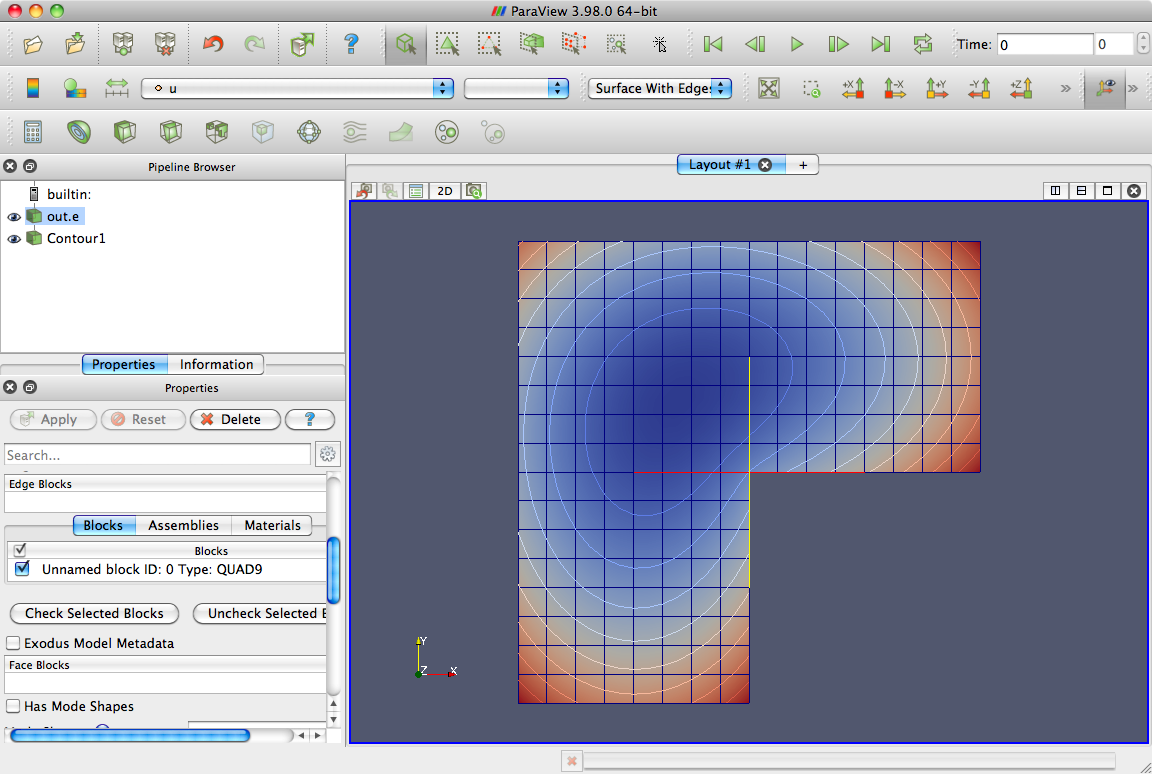
\includegraphics[height=0.8\textheight]{tutorial/laplace_young/screen}
  \end{center}
} 


\begin{frame}[fragile]
  \frametitle{Running the \texttt{transient\_convection\_diffusion} program}
    \begin{block}{Running the program}
    \begin{lstlisting}[language=bash]
# copy the example
$ cp -r $LIBMESH_TUTORIAL/transient_convection_diffusion .
$ cd transient_convection_diffusion
$ make

# run the example
$ ./example-opt
    \end{lstlisting}
  \end{block}
\end{frame}


\frame
{
  \frametitle{Output}
  \begin{center}
    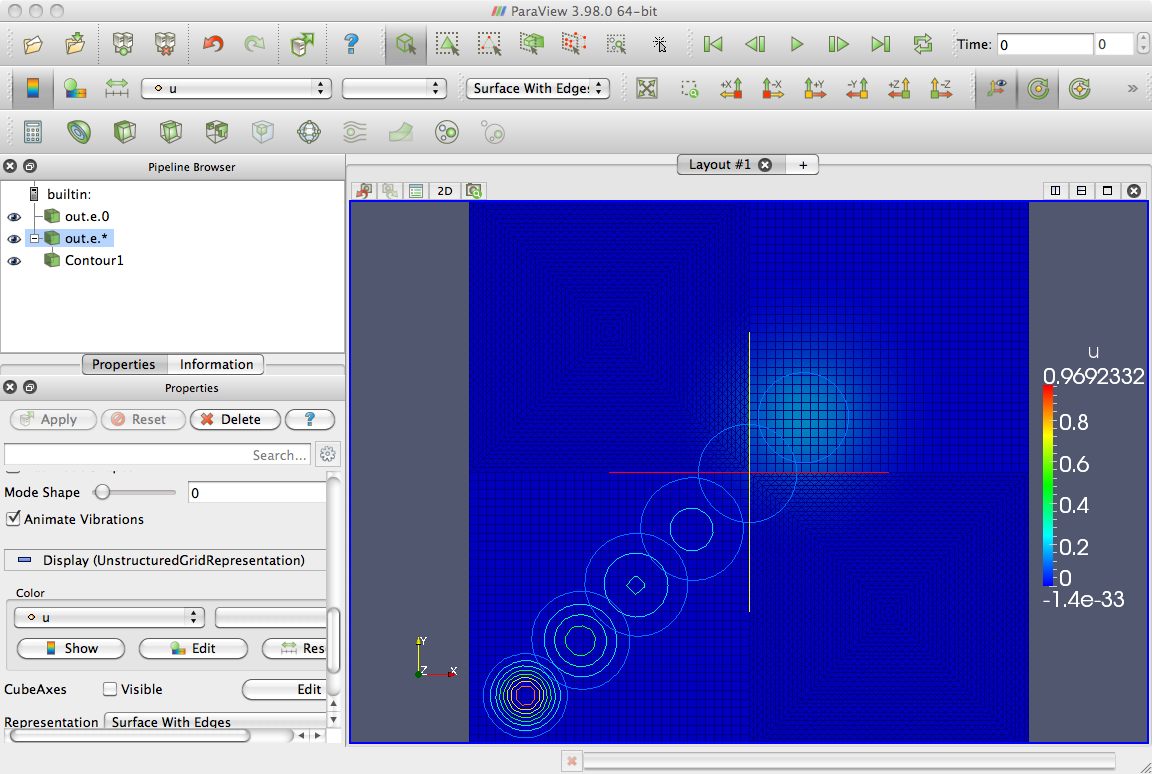
\includegraphics[height=0.8\textheight]{tutorial/transient_convection_diffusion/screen}
  \end{center}
} 
